%
%
\begin{figure}[ht]
  \begin{flushleft}
   \begin{tabular}{ll}
     \subfigure[KB03: $x/c=0.105$ suction side]
        {\hspace{-10mm}
         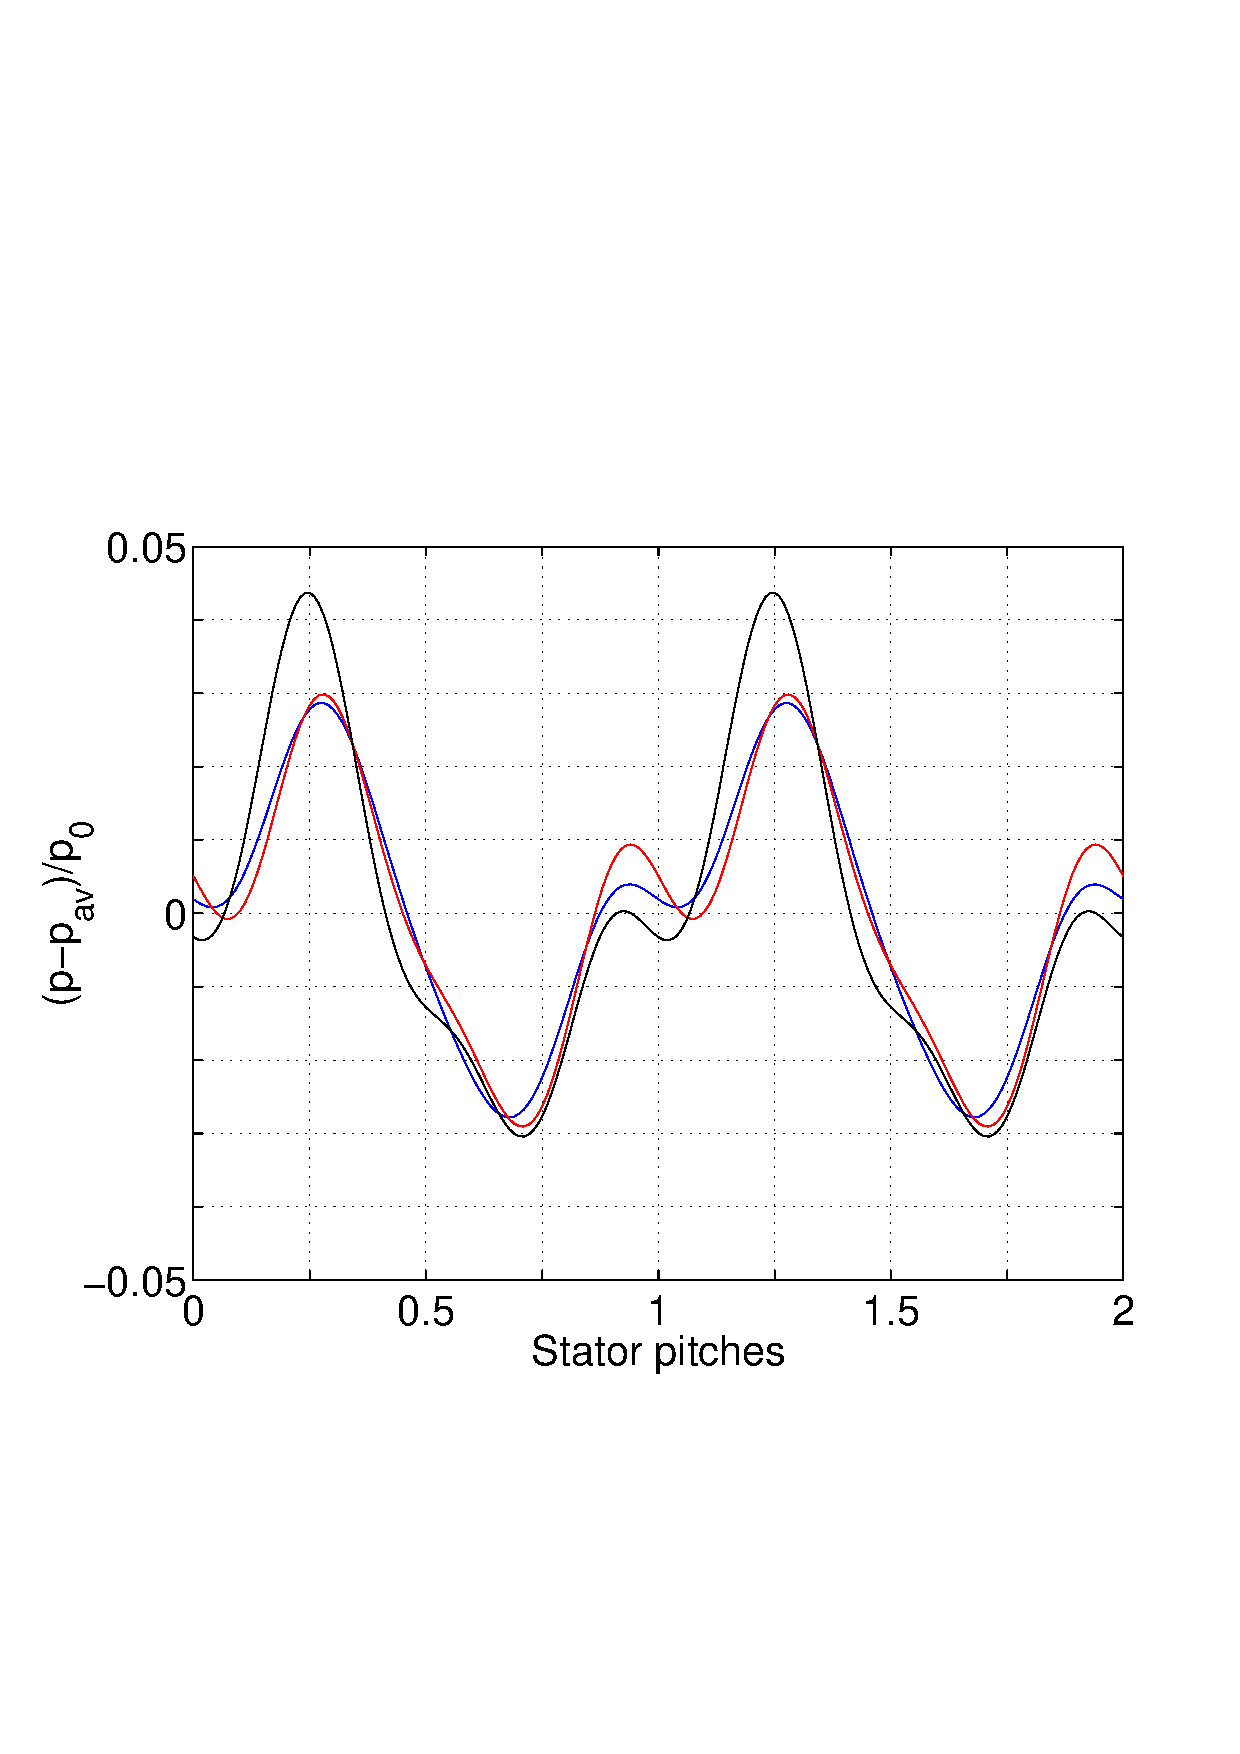
\includegraphics[width=75mm,clip=t]{CHAP_RT27/FIGURE/kb03.pdf}}
         &
     \subfigure[K003: $x/c=0.182$ suction side]
        {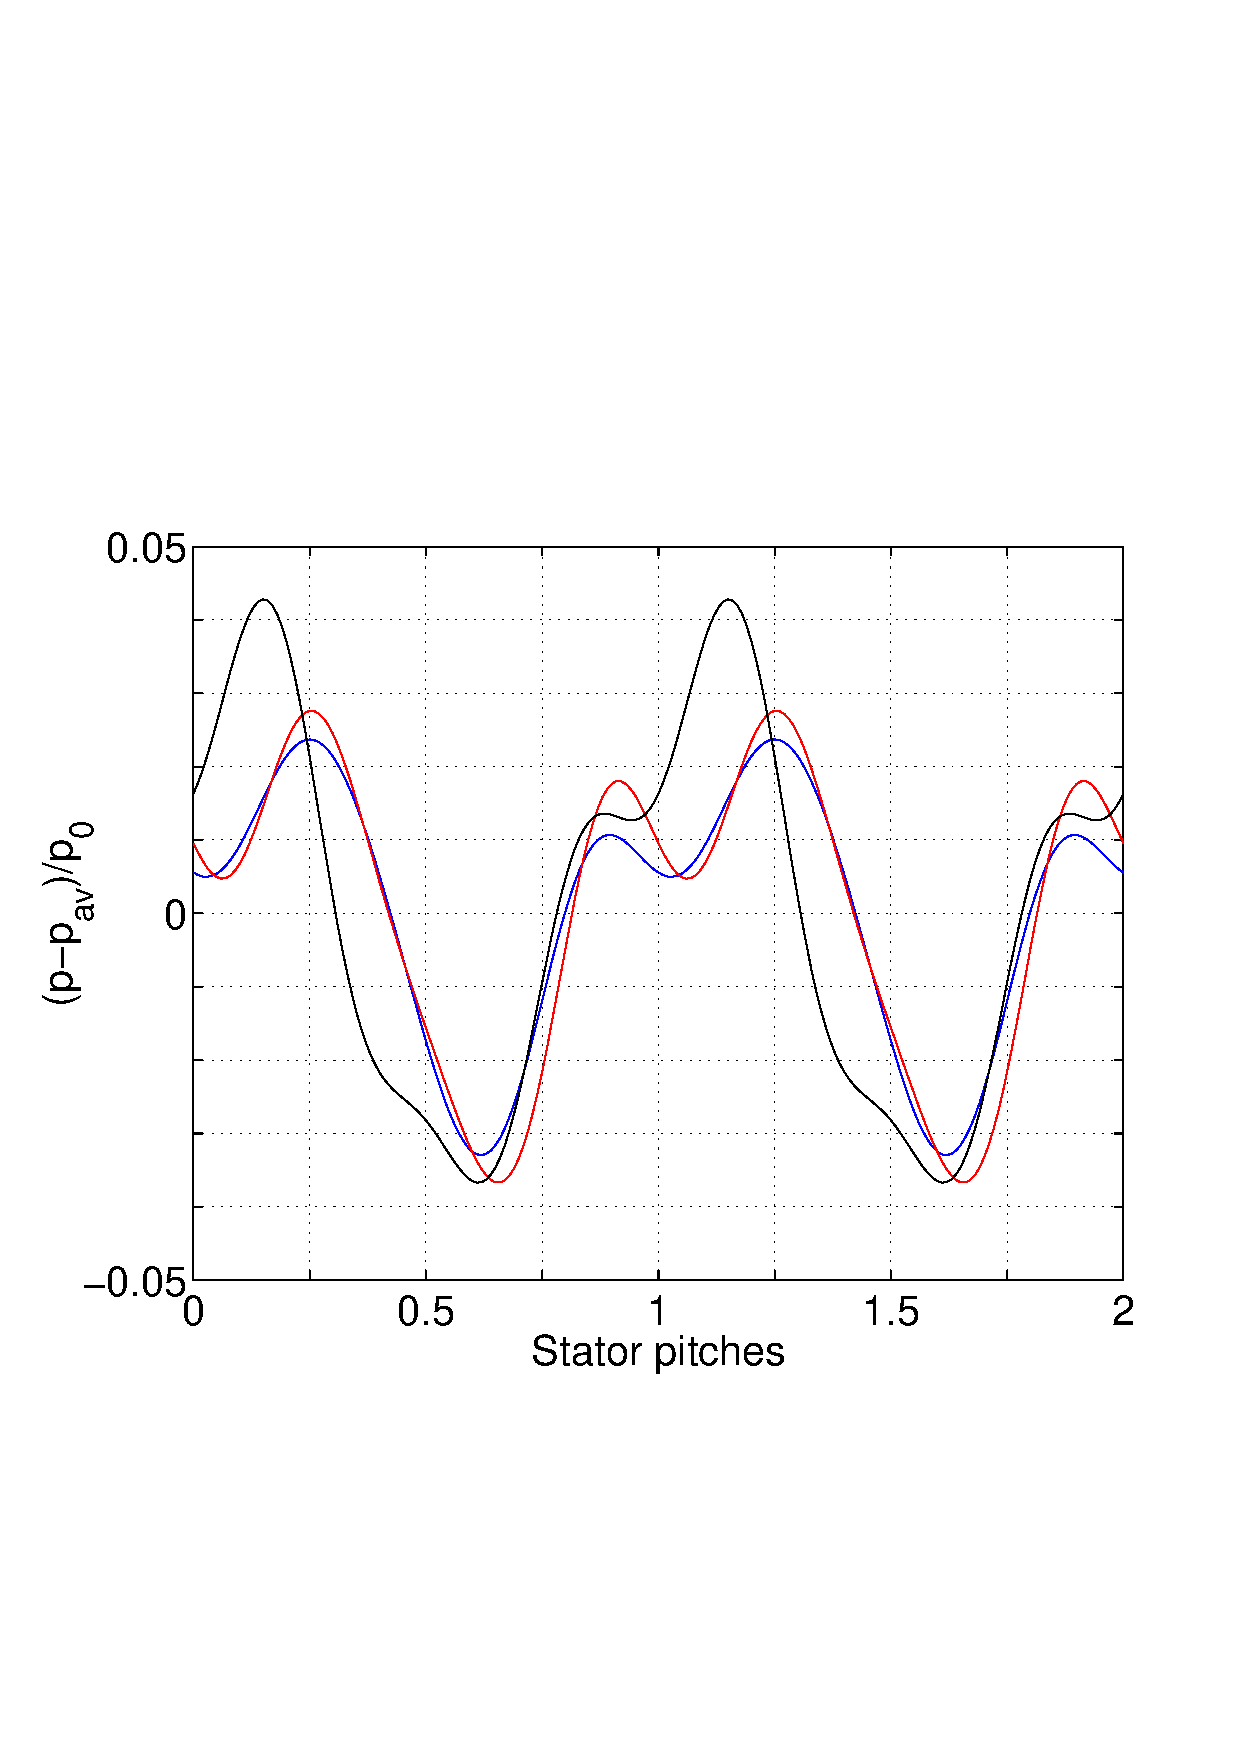
\includegraphics[width=75mm,clip=t]{CHAP_RT27/FIGURE/k003.pdf}}
         \vspace{-5mm}\\
     \subfigure[KB04: $x/c=0.250$ suction side]
        {\hspace{-10mm}
         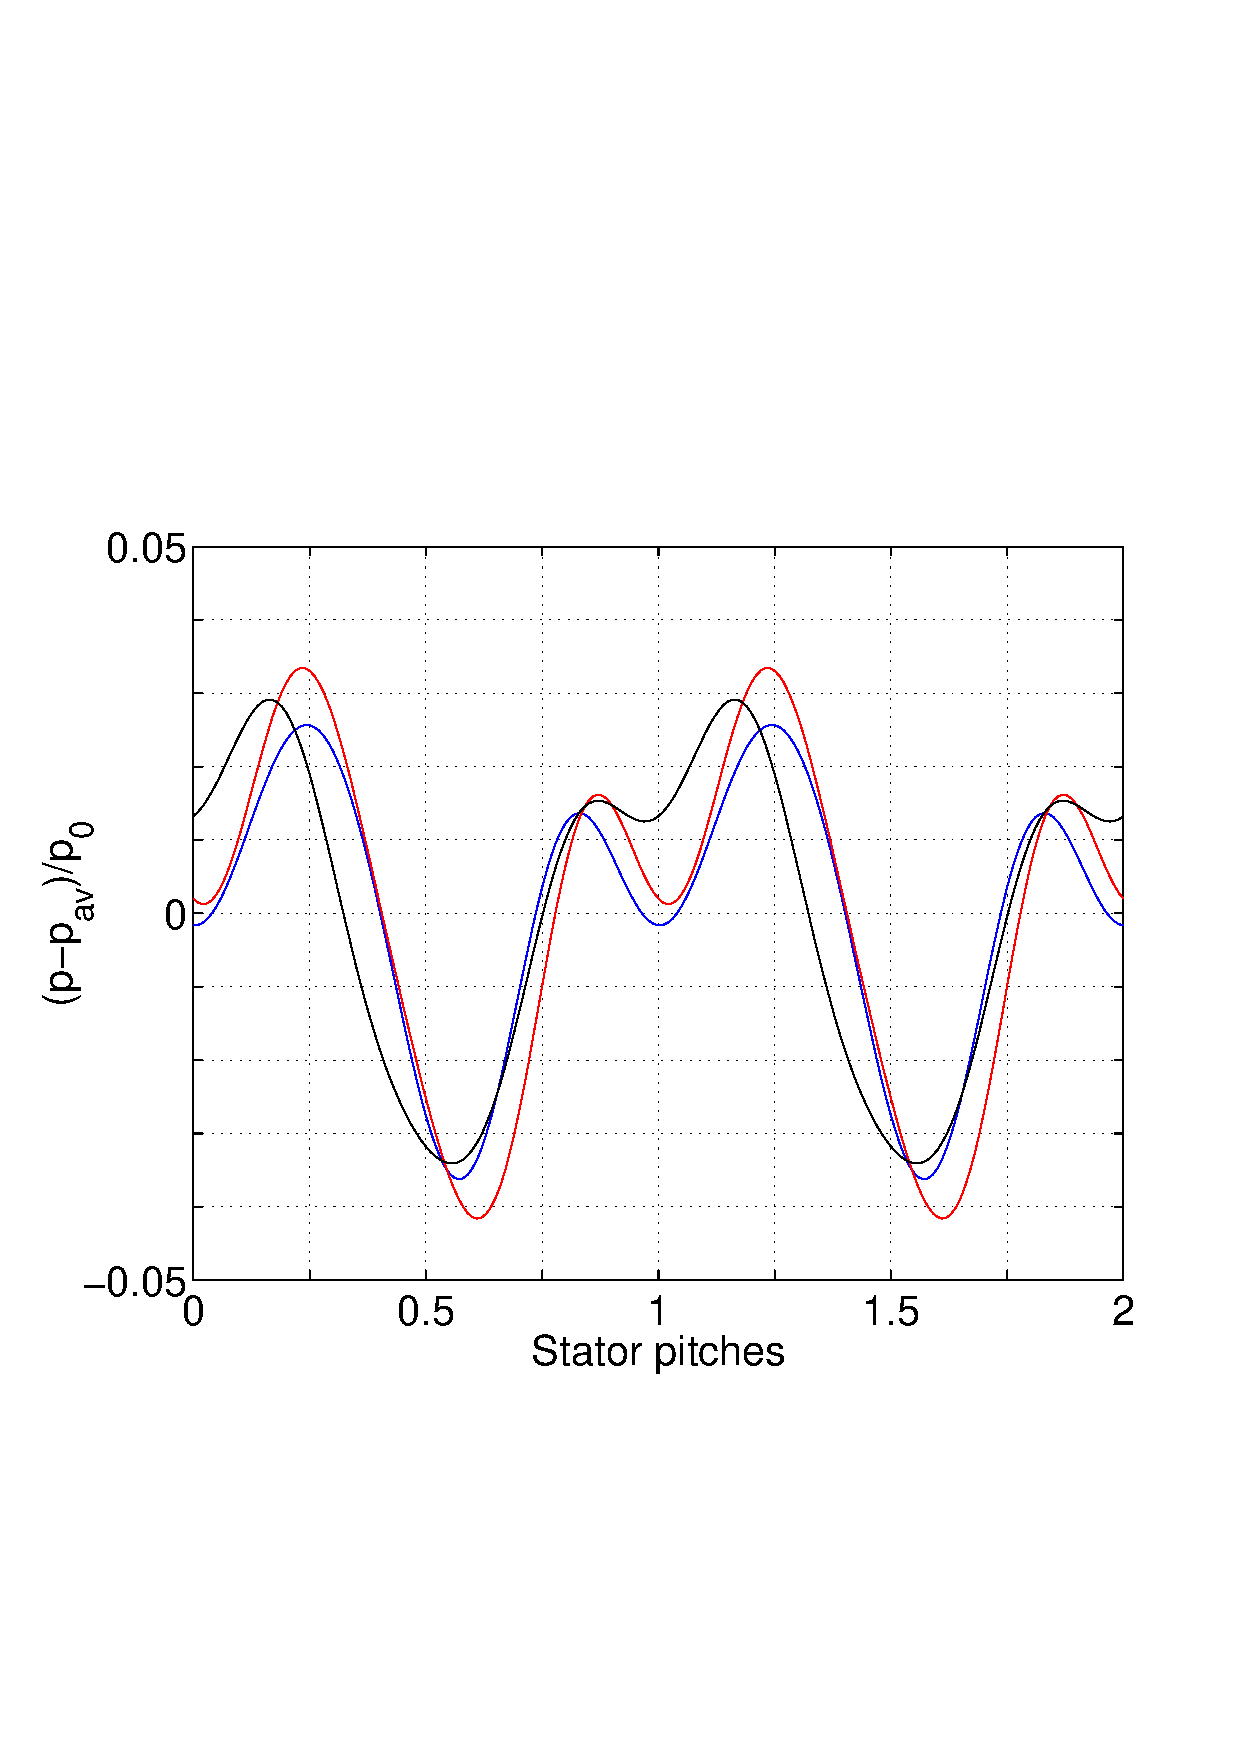
\includegraphics[width=75mm,clip=t]{CHAP_RT27/FIGURE/kb04.pdf}}
         &
     \subfigure[K005: $x/c=0.425$ suction side]
        {\includegraphics[width=75mm,clip=t]{CHAP_RT27/FIGURE/k005.pdf}}
         \vspace{-5mm}\\
     \subfigure[KB05: $x/c=0.460$ suction side]
        {\hspace{-10mm}
         \includegraphics[width=75mm,clip=t]{CHAP_RT27/FIGURE/kb05.pdf}}
         &
     \subfigure[K006: $x/c=0.518$ suction side]
        {\includegraphics[width=75mm,clip=t]{CHAP_RT27/FIGURE/k006.pdf}}
   \end{tabular}
  \end{flushleft}
  \vspace{-8mm}
  \caption{RT27A rotor blade mid-section.
   Comparison of unsteady pressure between
   linear results (blue), nonlinear results (red) and measured data (black)}
  \label{rt27_compar1.fig}
\end{figure}
%
%
%
\begin{figure}[ht]
  \begin{flushleft}
   \begin{tabular}{ll}
     \subfigure[K007: $x/c=0.588$ suction side]
        {\hspace{-10mm}
         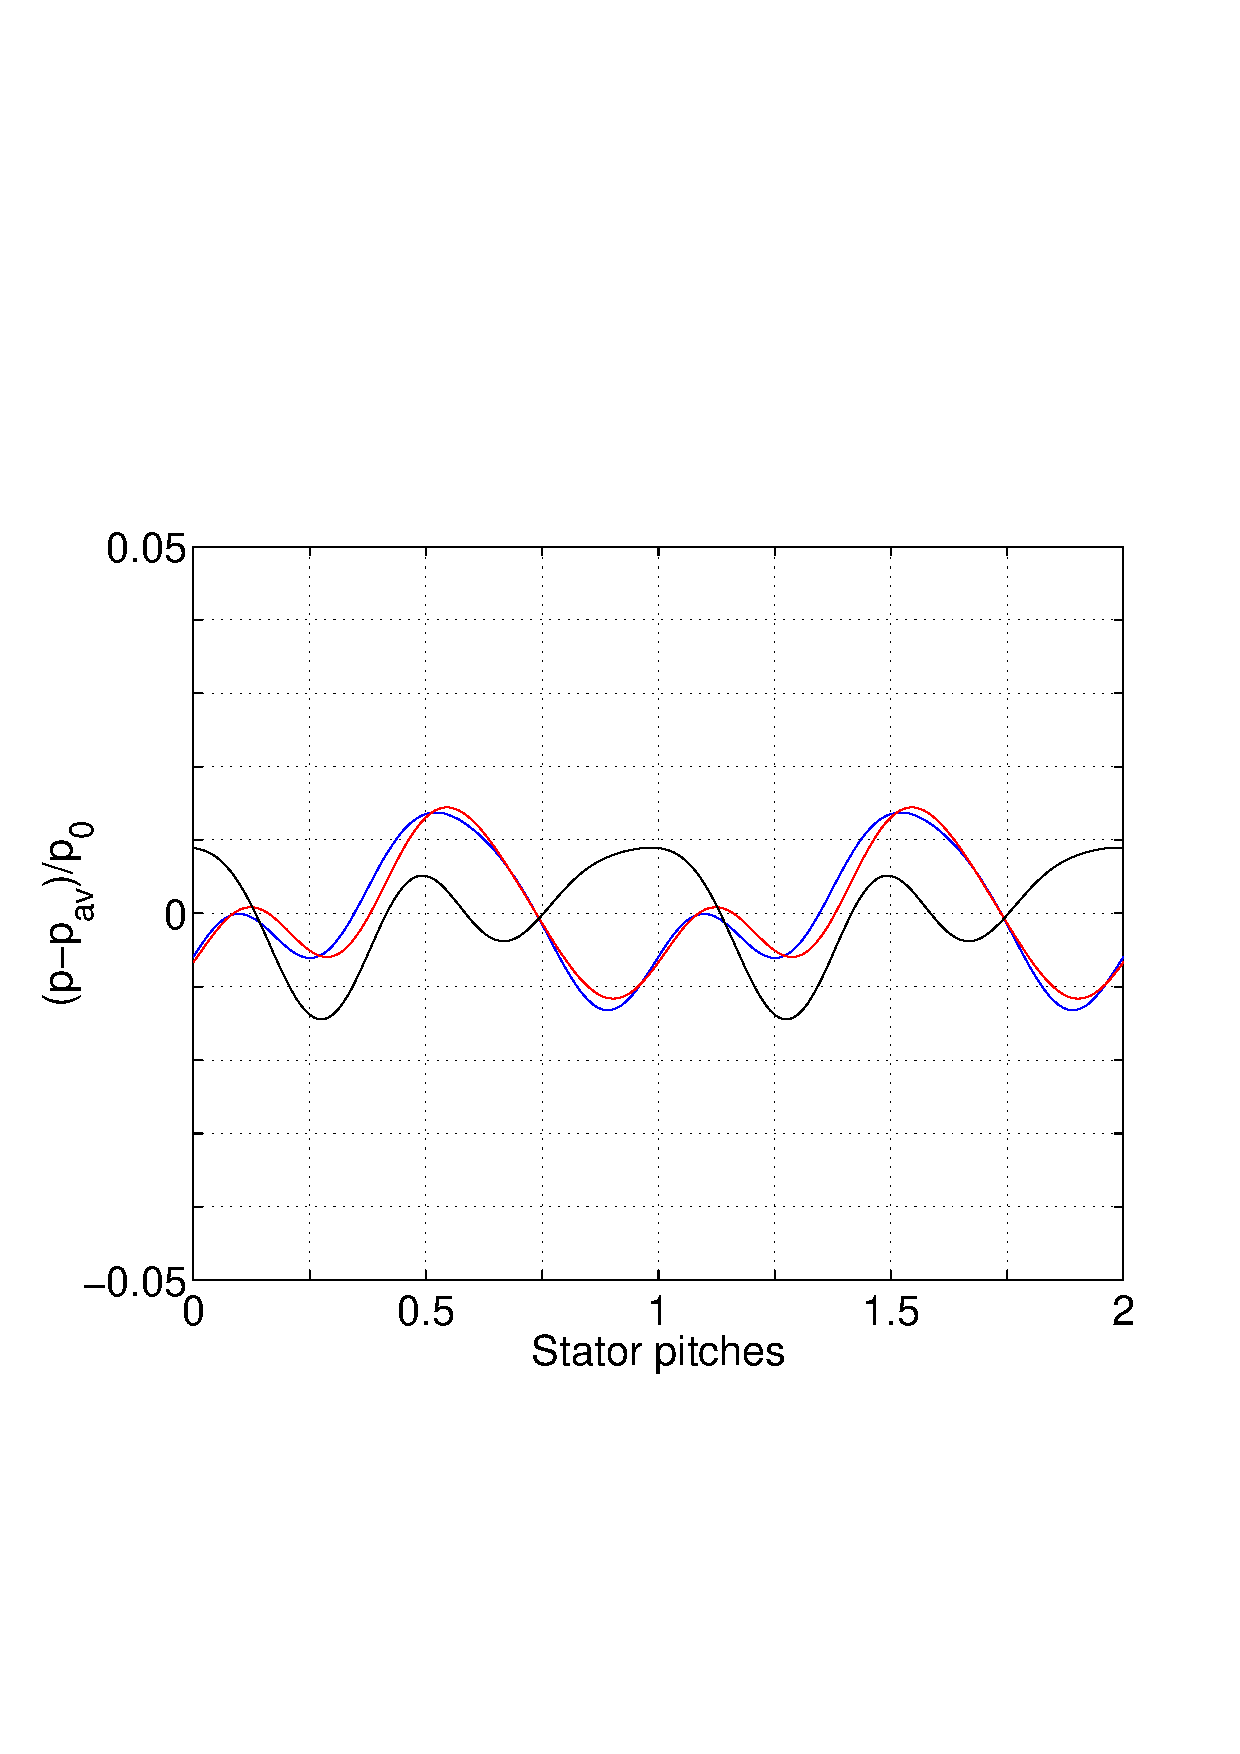
\includegraphics[width=75mm,clip=t]{CHAP_RT27/FIGURE/k007.pdf}}
         &
     \subfigure[K008: $x/c=0.648$ suction side]
        {\includegraphics[width=75mm,clip=t]{CHAP_RT27/FIGURE/k008.pdf}}
         \vspace{-5mm}\\
     \subfigure[KB07: $x/c=0.763$ suction side]
        {\hspace{-10mm}
         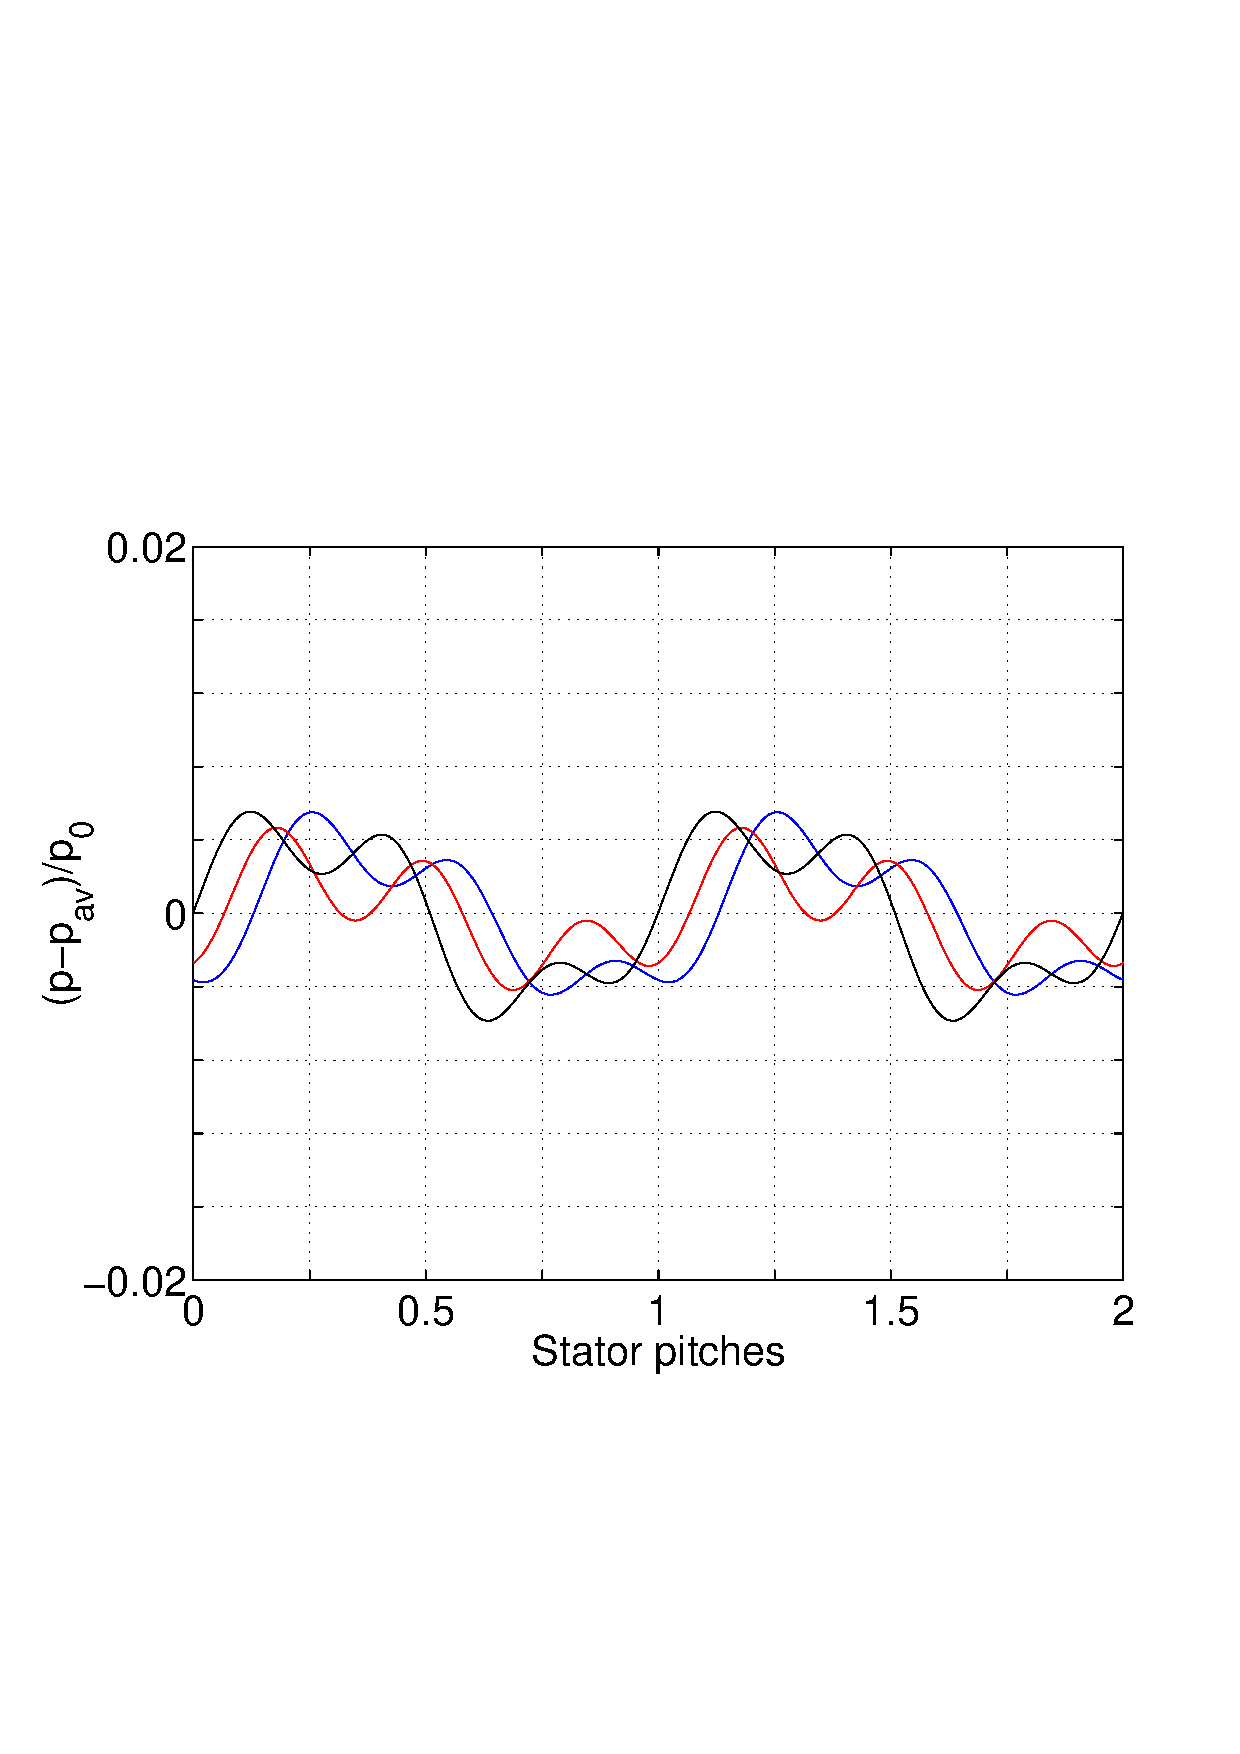
\includegraphics[width=75mm,clip=t]{CHAP_RT27/FIGURE/kb07.pdf}}
         &
     \subfigure[KB08: $x/c=0.886$ suction side]
        {\includegraphics[width=75mm,clip=t]{CHAP_RT27/FIGURE/kb08.pdf}}
         \vspace{-5mm}\\
     \subfigure[K014: $x/c=0.922$ suction side]
        {\hspace{-10mm}
         \includegraphics[width=75mm,clip=t]{CHAP_RT27/FIGURE/k014.pdf}}
         &
     \subfigure[K015: $x/c=0.975$ suction side]
        {\includegraphics[width=75mm,clip=t]{CHAP_RT27/FIGURE/k015.pdf}}
   \end{tabular}
  \end{flushleft}
  \vspace{-8mm}
  \caption{RT27A rotor blade mid-section (continued 1).
   Comparison of unsteady pressure between
   linear results (blue), nonlinear results (red) and measured data (black)}
  \label{rt27_compar2.fig}
\end{figure}
%
%
%
%
%
\begin{figure}[ht]
  \begin{flushleft}
   \begin{tabular}{ll}
     \subfigure[KA01: $x/c=0.055$ pressure side]
        {\hspace{-10mm}
         \includegraphics[width=75mm,clip=t]{CHAP_RT27/FIGURE/ka01.pdf}}
         &
     \subfigure[KA02: $x/c=0.143$ pressure side]
        {\includegraphics[width=75mm,clip=t]{CHAP_RT27/FIGURE/ka02.pdf}}
         \vspace{-5mm}\\
     \subfigure[KA04: $x/c=0.421$ pressure side]
        {\hspace{-10mm}
         \includegraphics[width=75mm,clip=t]{CHAP_RT27/FIGURE/ka04.pdf}}
         &
     \subfigure[KA06: $x/c=0.685$ pressure side]
        {\includegraphics[width=75mm,clip=t]{CHAP_RT27/FIGURE/ka06.pdf}}
         \vspace{-5mm}\\
     \subfigure[K102: $x/c=0.755$ pressure side]
        {\hspace{-10mm}
         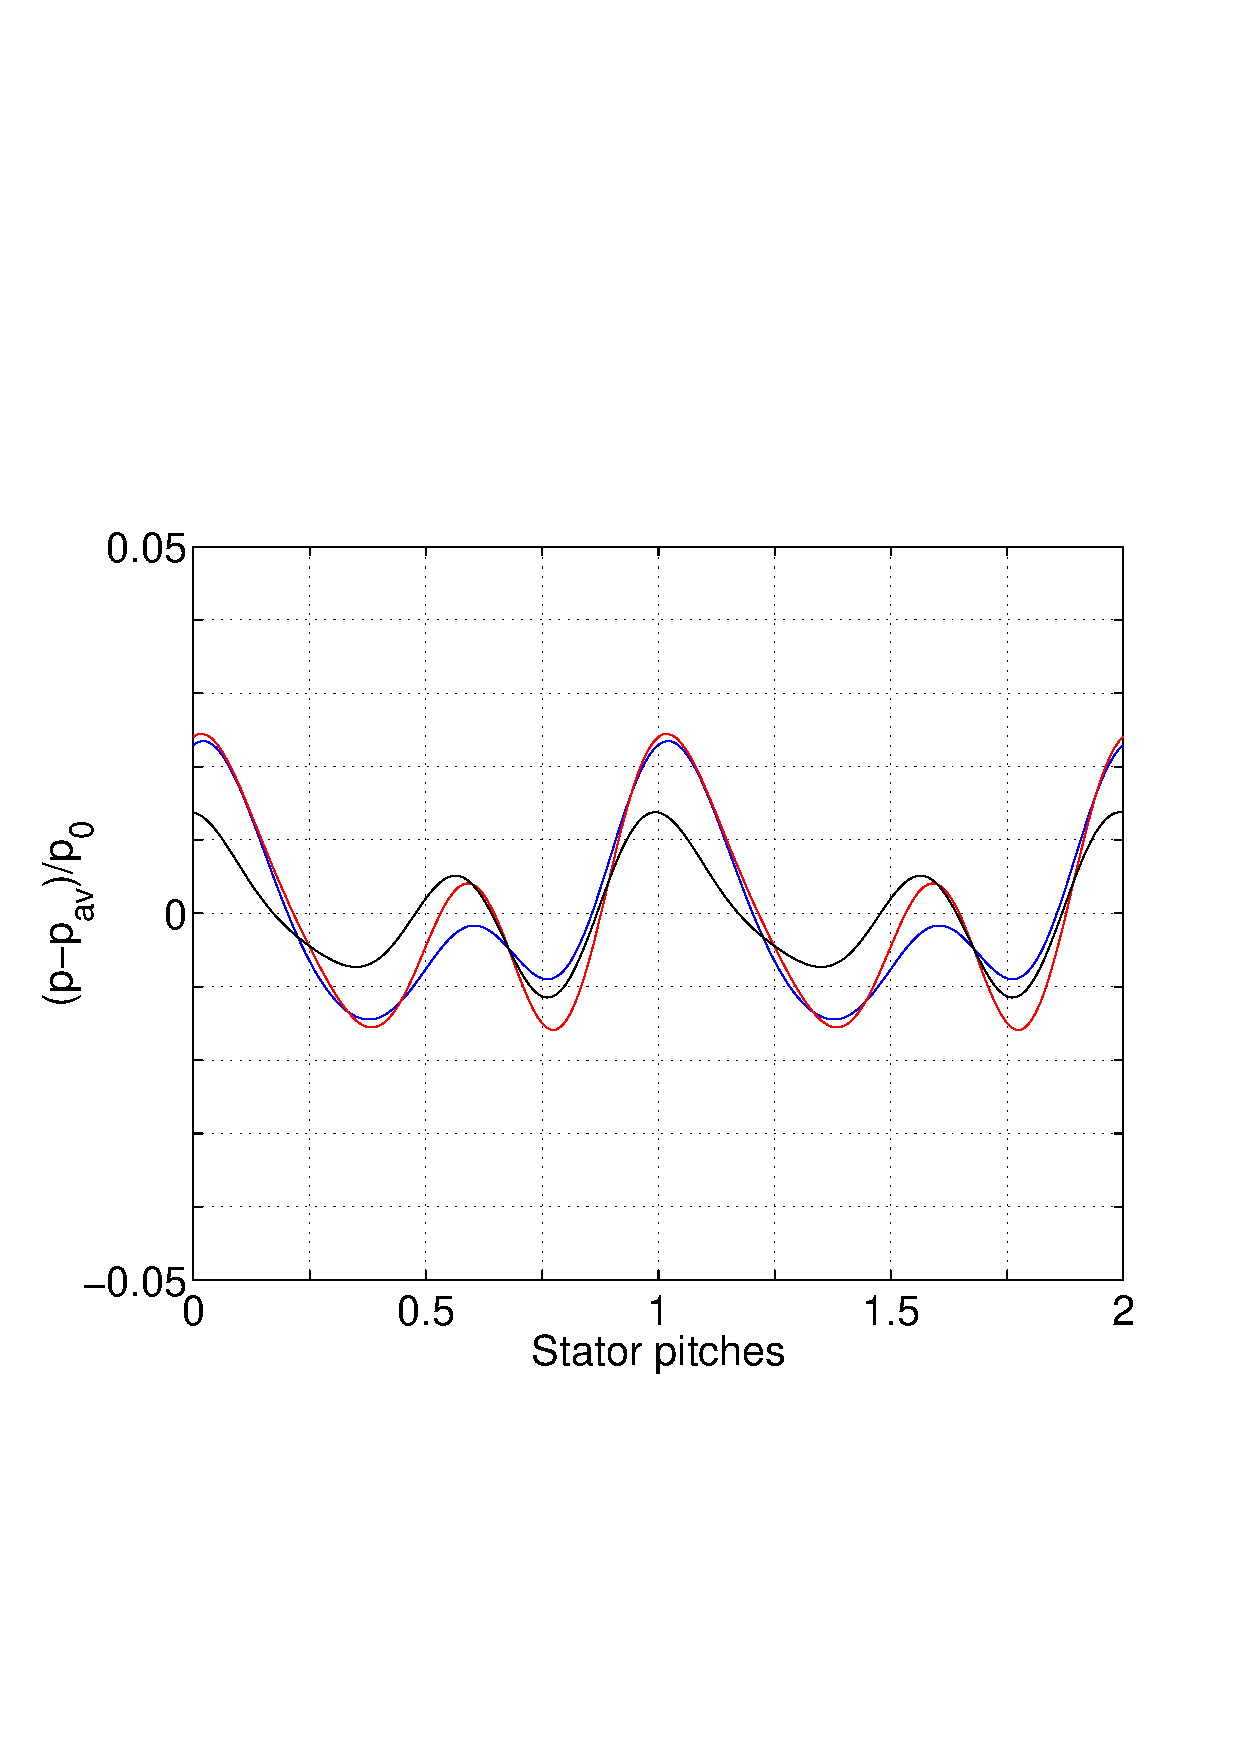
\includegraphics[width=75mm,clip=t]{CHAP_RT27/FIGURE/k102.pdf}}
         &
     \subfigure[KA08: $x/c=0.943$ pressure side]
        {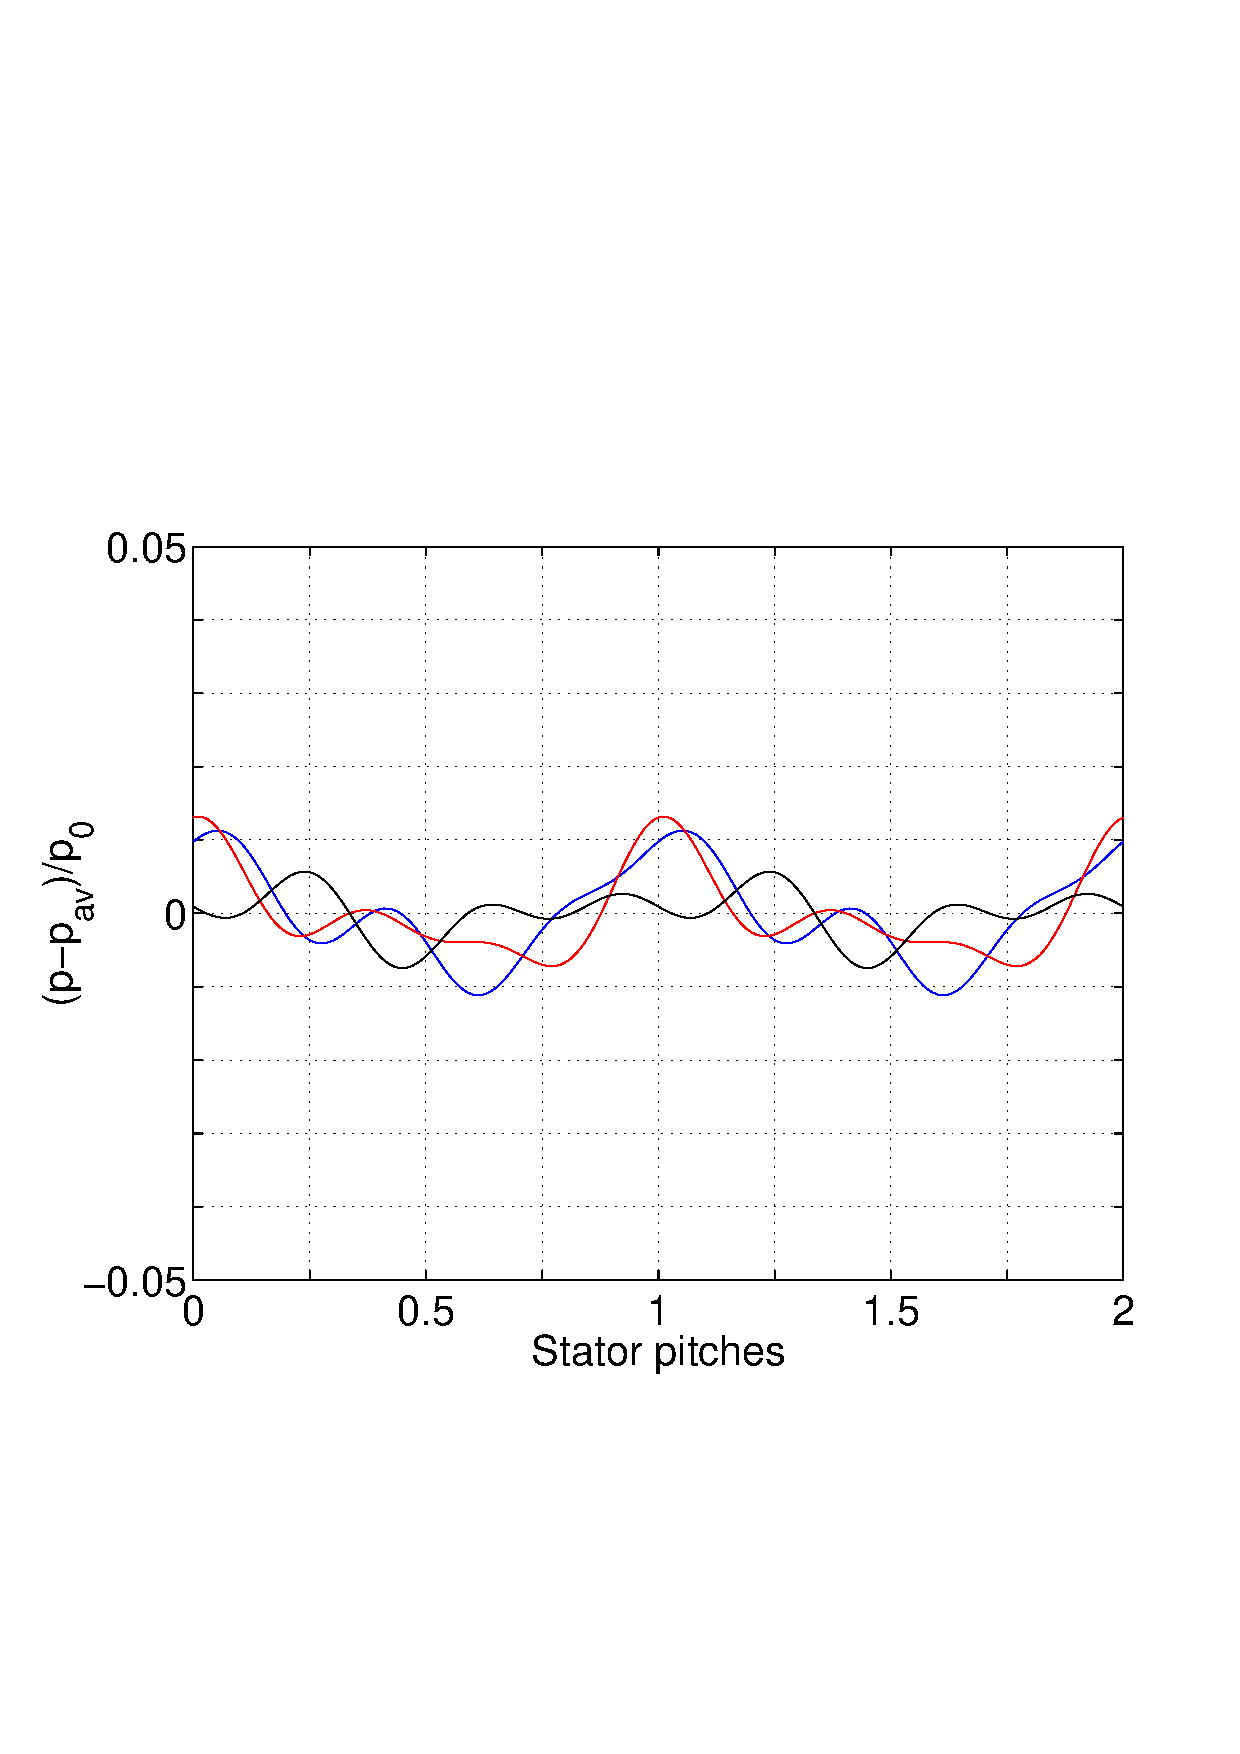
\includegraphics[width=75mm,clip=t]{CHAP_RT27/FIGURE/ka08.pdf}}
   \end{tabular}
  \end{flushleft}
  \vspace{-8mm}
  \caption{RT27A rotor blade mid-section (continued 2).
   Comparison of unsteady pressure between
   linear results (blue), nonlinear results (red) and measured data (black)}
  \label{rt27_compar3.fig}
\end{figure}
%
%
